\chapter{Tests des structures d'égalisation DFVE}

\paragraph{}
Nous devions vérifier expérimentalement deux structures d'égalisation DFVE (temporelle et fréquentielle). Dans ce chapitre, nous aurons connaissance du canal de propagation à la réception, sans l'utilisation des pilotes. Nous avons donc crée un signal OFDM, modélisé l'effet du canal de propagation, et ensuite nous avons testé les deux structures d'égalisation DFVE en connaissant la réponse du canal, et donc sans algorithme d'éstimation des coefficients complexes (Chapitre suivant). Les codes MATLAB commentés sont disponible avec ce rapport.

\section{Création du signal}

\paragraph{}
Nous avons choisi de prendre 4 sous-porteuses avec la première à 2.412 GHz, et les suivantes espacée de 0.3125MHz afin du simulé 4 sous-porteuses du canal 1 du WIFI en France. Nous avons choisi comme modulation, une $\pi/4$-DPSK dont un état représente le chiffre 1, un autre le 2, puis le 3 et le 4. Ensuite nous créeons aléatoirement un vecteur de ces 4 chiffres, et le modulons. Nous pouvons voir le diagramme de constellation sur la Figure ~\ref{QPSK}.

\paragraph{}
\vspace{1\baselineskip}
\begin{figure}[!h]
  \centering
  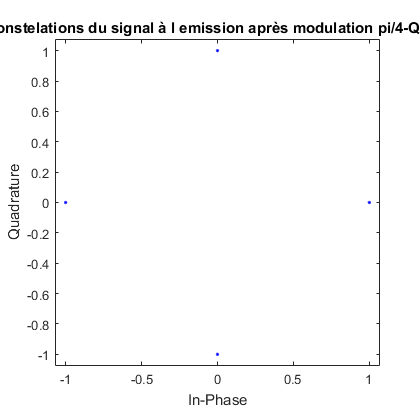
\includegraphics[scale=0.6]{QPSKdep.png}
  \caption{Diagramme de constellation avant l'IFFT }
	\label{QPSK} 
\end{figure}
\vspace{10\baselineskip}

\paragraph{}
Ensuite, nous créeons notre signal après en avoir effectué l'IFFT. Nous obtenons le signal visible sur la Figure ~\ref{signal}.

\paragraph{}
\vspace{1\baselineskip}
\begin{figure}[!h]
  \centering
  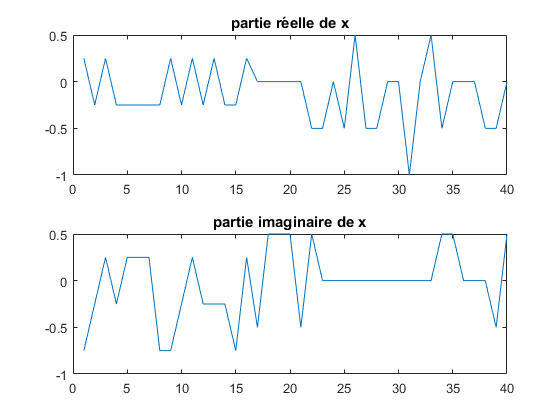
\includegraphics[scale=0.6]{signalSR.png}
  \caption{Signal à la sortie du récepteur }
	\label{signal} 
\end{figure}
\vspace{1\baselineskip}

\section{Canal de propagation}
\paragraph{}
Nous avons modélisé la réponse fréquentielle du canal par le filtre d'un canal écho de fonction de transfert $H(f)=1+(0.4+j*0.2)*f^{-1}$. Sur la Figure ~\ref{fonctionT}, nous pouvons voir la réponse en gain et en phase du canal.
\paragraph{}
\vspace{1\baselineskip}
\begin{figure}[!h]
  \centering
  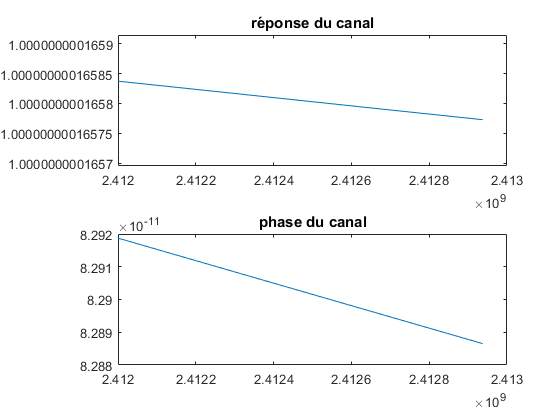
\includegraphics[scale=0.8]{fonctionT.png}
  \caption{Réponse fréquentielle du canal sur la bande du signal OFDM}
	\label{fonctionT} 
\end{figure}
\vspace{1\baselineskip}
\paragraph{}
Ensuite nous convoluons notre signal temporelle par la réponse fréquentielle du canal, puis nous ajoutons un bruit Gaussien complexe de variance 0.01. Notre signal est ainsi transformé comme nous pouvons le voir sur la Figure ~\ref{ajoutCanal} 
\paragraph{}
\vspace{1\baselineskip}
\begin{figure}[!h]
  \centering
  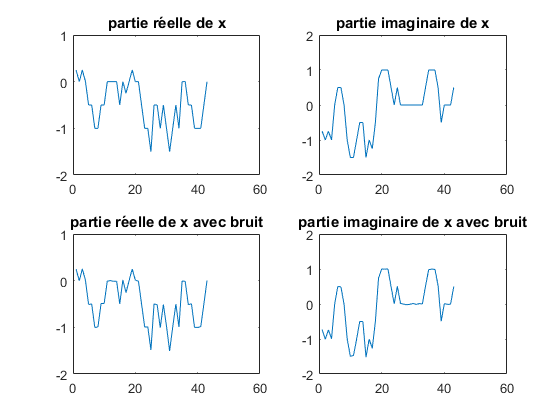
\includegraphics[scale=0.8]{ajoutCanal.png}
  \caption{Signal à l'entrée du récepteur sans bruit et avec bruit}
	\label{ajoutCanal} 
\end{figure}
\vspace{1\baselineskip}


\section{Structure fréquentielle DFVE}


\section{Structure temporelle DFVE}






%%% Local Variables:
%%% mode: latex
%%% TeX-master: "../rapport_de_base"
%%% End:
